\chapter{Knowledge Graph Embeddings}\label{chap:embeddings}

\chapterQuote{\textit{``Computer Science is a science of abstraction -creating the right model for a problem and devising the appropriate mechanizable techniques to solve it''}}{--- Alfred Aho}

%REESTRUCTURAR EN BASE A LOS COMENTARIO DE DANI, UNA EXPLICACION GENERAL SOBRE LO QUE SON Y LUEGO LOS DIFERENTES METODOS EN LOS QUE SE OBTIENEN.

% A mí esta sección me extrañó un poco en la tesis de Agu, ya que "tensor factorization" y "translational models" son los dos embeddings que se obtienen con redes neuronales. Yo hubiera explicado primero que un embedding es cualquier tipo de representación numérica que de alguna manera contenga información sobre la cosa representada. Y luego pondría (estructurado como sea más conveniente) que se puede hacer una representación con

% 1) Cualquier medición hecha sobre el nodo o relación. Por ejemplo si los nodos son documentos, su vector de embeddings podría ser la representación como bolsa de palabras.

% 2) Técnicas basadas en redes neuronales, que ajustan unos embeddings para que funcione la tarea de alguna red neuronal. Por ejemplo, una red neuronal que determine si dos nodos están unidos o no. Como esto depende de lo que representen los nodos y sus características, pues al final los embeddings de alguna manera reflejan lo que representen los nodos y sus características. Estas técnicas tienen la ventaja de que son aplicables a los nodos de cualquier grafo, includo si hay varios tipos de nodos.

\chapterAbstract{R}{epresenting the information in knowledge graphs in a way that is usable for machine learning techniques became one of the main focuses of research after their inception. The inception of these representations flourished from several KG completion techniques with numerical vectors representing the entities and relations of the KG as a byproduct of them. In this chapter, we evolutionarily introduce several of these techniques. It is structured as follows: Section~\ref{sec:emb-intro} provides an introduction to the matter, Section~\ref{sec:emb-translations} introduces the methods that leverage translation operations, Section~\ref{sec:emb-semantic} elaborates on the methods which focus on matching information semantically, Section~\ref{sec:emb-tensor} discusses the proposals which focus on the use of tensor representations of the KG; Section~\ref{sec:emb-nn} overviews the methods which make use of neural network in their approaches, and finally, Section~\ref{sec:emb-summary} provides a summary of the contents of the chapter.
}

\section{Introduction}\label{sec:emb-intro}
Embeddings are a form of representation of information which gathers the semantic, contextual, relational and modular data within an information node and converts it into a numerical representation, as a N-dimensional vector.

In particular KG embeddings represent the nodes and relations in the graph which can be captured either semantically with a bag of words vector, positionally with one one of the mutiple techniques described, or with a combined approach, an enriched positional vector.

Knowledge graph embeddings aid in representing information within a KG in a way that is understandable for Machine learning tasks. These embeddings provide a compact, continuous vector representation for entities and relationships, allowing for efficient computational operations and meaningful interpretations.

These vectors capture the semantic nuances of the entities and the connections between them. In essence, knowledge graph embeddings serve as a bridge between the discrete, symbolic world of knowledge graphs and the continuous, numerical space of machine learning algorithms.

The process of obtaining knowledge graph embeddings involves mapping entities and relationships to low-dimensional vector spaces. This transformation is designed to preserve the essential structural and semantic information of the knowledge graph. Entities are represented as points in this vector space, while relationships are encoded as transformations that operate on entity vectors.

The goal is to position entities and relationships in such a way that their geometric relationships in the embedding space reflect the underlying semantic relationships in the knowledge graph. In this manner, knowledge graph embeddings serve as a powerful tool for capturing the rich tapestry of connections, dependencies, and contextual information present in knowledge graphs.

Along the following sections the following nomenclature will be followed, where, ``h'' denotes a head entity, ``r'' denotes the relation that connects them and ``t'' denotes a tail entity making (h, r, t) a triple in the graph. $\mathcal{E}$ is the set of all entities and $\mathcal{R}$ is the set of all relations in the graph.

\section{Translation models}\label{sec:emb-translations}

% \todo{table with the evolution of the proposals, as an overview?}

Translation models usually use distance-based functions to define the scoring function for link prediction tasks, the general idea behind these models is that if we apply a translation operation based on a relation ``r'' to an entity ``h'' represented by a low dimensional vector the result should be close to its destination entity ``t'' in the triple (h, r, t) which is considered correct as it is in the graph.

TransE \cite{} is a well-known, early and simple model that regards a relation as a translation from a head entity to a tail entity, used for link prediction it generates embeddings representations for entities and relation in KGs, it uses the relation representation to apply a translation from the head entity to a tail entity. It considers the uncertainties of entities and relations by using a probability function. 

\begin{figure}[!htp]
    \centering
    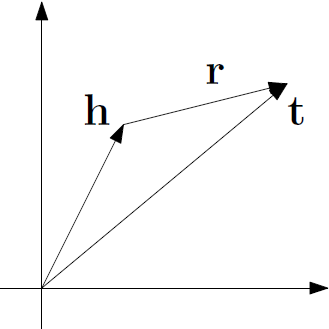
\includegraphics[width=.4\textwidth]{fig/embeddings/TransE.png}
    \caption{TransE representation in 2D Space}
    \label{fig:emb-transE}
\end{figure}

The basic idea behind this model is that the connecting relation between the two entitiy representations makes it so  $h + r \approx t$ as shown by the figure \ref{fig:emb-transE}, It uses the distance scoring function defined by \ref{eq:transE_scoring} accordingly.

\begin{equation}
    \label{eq:transE_scoring}
    f (h, t) = ||h + r - t||_1
\end{equation}
    
TransE is the earliest translation-based embedding model, and it has difficulty dealing with multirelational graphs; it is limited by its simple translation operation as well as its lack of a discrimination policy for all kinds of relations.

Improving on TransE, TransH introduces the concept of hyperplanes translations, in order to overcome the problems of TransE in modeling reflexive multiorigin or multidestination relations (one-to-many, many-to-one, many-to-many)this model enables an entity to have distributed representations when involved in different relations. 

\begin{figure}[!htp]
    \centering
    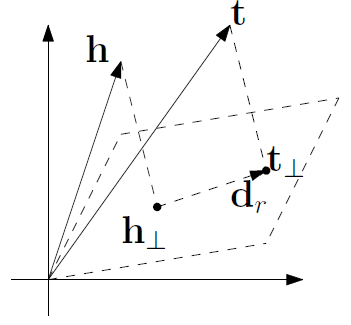
\includegraphics[width=.4\textwidth]{fig/embeddings/TransH.png}
    \caption{TransH representation in 2D Space}
    \label{fig:emb-transH}
\end{figure}

As illustrated in Figure \ref{fig:emb-transH}, the relation translation vector $d_r$ is contained within the plane rather than being connected directly such as in TransE.

for a triple (h, r, t), the embedding h and t are first projected to the plane ($h\bot$, $t\bot$). They are then connected by a translation vector $d_r$ in the hyperplane. The scoring funtion is described as by \ref{eq:transH_scoring}

\begin{equation}
    \label{eq:transH_scoring}
    f (h, t) = || (h - w^\tau_r |hw_r) + d_r - (t-w^\tau_r tw_r) ||^2_2
\end{equation}
\begin{center}
    $w_r, d_r \in \mathbb{R}$
\end{center}

Improving on then TransH model appears TransR\cite{} which innovates by using a relation-specific space to handle different relations. As an entity may have multiple semantical interpretations different relations focus on different ones. TransR models entities and relations in distinct spaces, entity and relation spaces and performs translation in the corresponding relation space.

\begin{figure}[!htp]
    \centering
    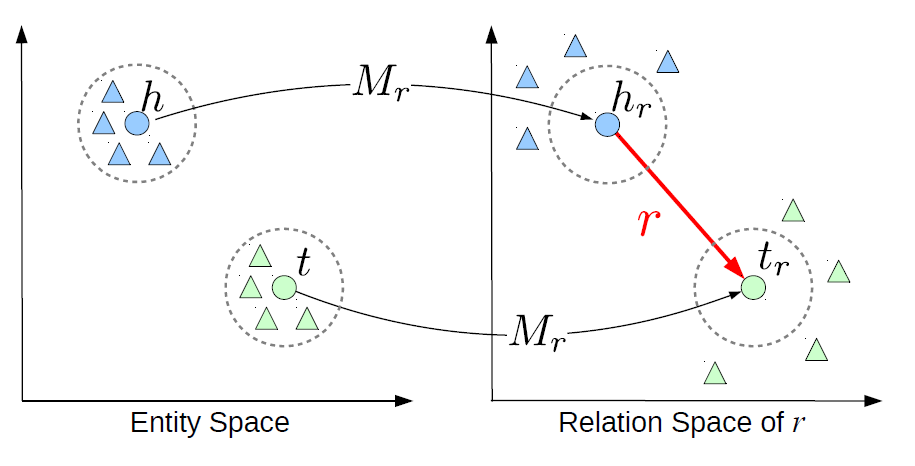
\includegraphics[width=.7\textwidth]{fig/embeddings/TransR.png}
    \caption{TransR representation in 2D Space}
    \label{fig:emb-transR}
\end{figure}

Figure \ref{fig:emb-transR} shows a simple rendition for the TransR model, it depicts how for a given triple (h, r, t), entities ``h'' and ``t'' are projected into the relation space for relation ``r'', then a translation is performed in said vectorial space. This relation specific space also shows how other entities appear further away from the source triple as they are not close semantically for that particular relation space. TransR scoring function \ref{eq:transR_scoring} is very closely related to TransE scoring function with the key difference that is performed in a diferent space.

\begin{equation}
    \label{eq:transR_scoring}
    f(h, t) = ||h_r + r - t_r||^2_2
\end{equation}

Several iterations of the Trans(+letter) model have been proposed as improvements to these previously mentioned approaches, all of them iterating on the idea of decoupling entity and relations interactions to then perform a translation operation of some sort.

To conclude this section RotatE\cite{} presents an improvement from previous techniques by defining each relation as a rotation from the ``h'' to ``t'' in a complex plane and the same vector space as shown in figure \ref{fig:emb-rotatE}.

\begin{figure}[!htp]
    \centering
    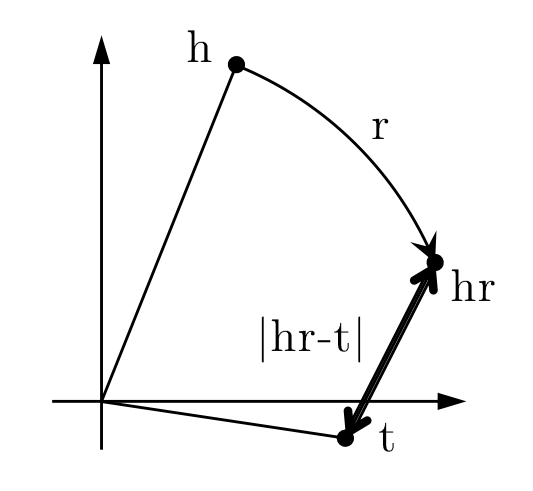
\includegraphics[width=.4\textwidth]{fig/embeddings/RotatE.png}
    \caption{RotatE in a 2D plane}
    \label{fig:emb-rotatE}
\end{figure}

RotatE maps the head and tail entities ``h'' and ``t'' to complex embeddings then, it defines a mapping function induced by each relation ``r'' as an rotation from ``h'' to ``t'' where $t = h \circ r, where |r_i| = 1$ and $\circ$ is the Hadmard product.
By defining each relation as a rotation in the complex vector spaces, RotatE can model and infer relation patterns such as symmetry/antisymmetry, inversion and composition. 

\begin{equation}
    \label{eq:rotatE_scoring}
    f(h, t) = ||h \circ r - t||
\end{equation}

The distance function of RotatE \ref{eq:rotatE_scoring} corresponds to a counterclockwise rotation by $\theta_r,i$ radians about the origin of the complex plane, and only affects the phases of the entity embeddings in the complex vector space.

\section{Semantic information models}\label{sec:emb-semantic}
Semantic information-based models usually use similarity-based functions to define scoring functions for traditional semantic-matching models or introduce additional information to mine more knowledge for recently proposed models.

Traditional models match the latent semantics of entities and relation embeddings to measure the plausibility of a triple, however, these models suffer from high computational complexity.

More recent models fuse various additional information to obtain better performance to mine deeper semantic informationat the bottoms of graphs. The additional information includes path information, order information, concepts, entity attributes, entity types and so on.

Word2vec\cite{} goal is learning high-quality word vectors from huge data sets with billions of words, and with millions of words in the vocabulary by using distributed representations of words learned by neural networks following stochastic gradient descent methods and backpropagation.

\begin{figure}[!htp]
    \centering
    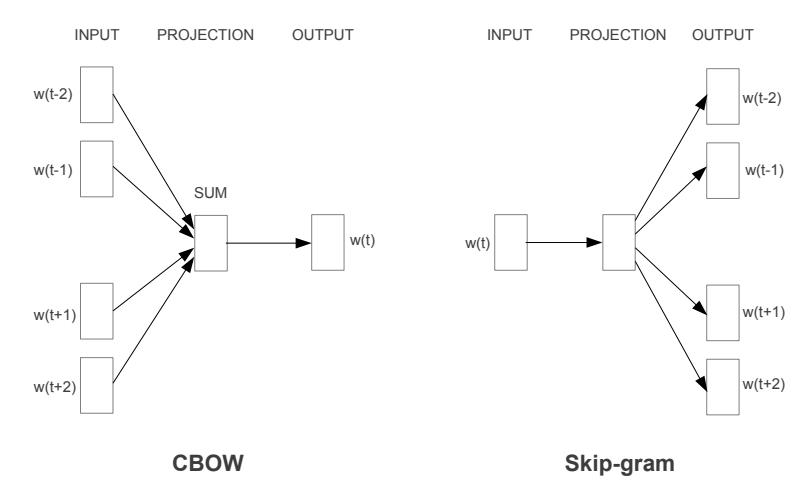
\includegraphics[width=.75\textwidth]{fig/embeddings/Word2Vec.png}
    \caption{Word2Vec models}
    \label{fig:emb-rotatE}
\end{figure}

It consist of two methods, a continuos bag-of-words model and a skip-gram model. The first of the two closely resembles a feedforward NNLM (Neural Network Language Model), where the projection intermediate layer is altered by all words in the input, therefore, all words alter the composition of the NN and their vectors are averaged.

The second model tries to maximize the classification of a word based on the sentence it is contained within. the entire context sentece is fed into a log-linear classifier which tries predict words before and after the current word.

GlovE \cite{} appears as a model able to capture a global corpus of words  statistics directly by using global matrix factorization and local context window methods. It is designed to capture semantic relationships between words by learning vector representations that encode the statistical information of word co-occurrence in a large corpus.

GloVe has become a popular choice for word embeddings in NLP due to its effectiveness in capturing semantic relationships and its relatively efficient training process.

GloVe starts by constructing a word co-occurrence matrix based on a given corpus. Each entry (i, j) in the matrix represents the number of times word i co-occurs with word j within a certain context window.

Then it trains in order to learn vector representations such that the dot product of these vectors corresponds to the logarithm of the observed word co-occurrence probabilities. The objective function of GloVe aims to minimize the difference between the dot product of word vectors and the logarithm of the co-occurrence probabilities.

The learned vectors represent words in a continuous vector space, where the distance and direction between vectors capture semantic relationships. Words with similar meanings or that often appear in similar contexts will have similar vector representations.

GloVe has been praised for its ability to capture meaningful semantic relationships between words. The resulting word embeddings often exhibit interesting properties, such as linear relationships that represent semantic analogies (e.g., "king" - "man" + "woman" $\simeq$ "queen").


\section{Tensor Factorization models}\label{sec:emb-tensor}
Tensor factorization try to solve KG completion tasks by relying on the fact that a Knowledge Graph can be represented as tensors where the relational data can be represented as a {0, 1}-valued third-order tensor Y, and, if a relation (h, r, t) is true it meets $Y_{h,r,t} = 1$, KGC can be framed as a 3rd-order binary tensor completion problem.

The first apporach to take advantage of the tensors being able to represent a Knowledge Graph was RESCAL \cite{}, which takes the inherent structure of relational data into account by operating over this tensor representation of.

\begin{figure}[!htp]
    \centering
    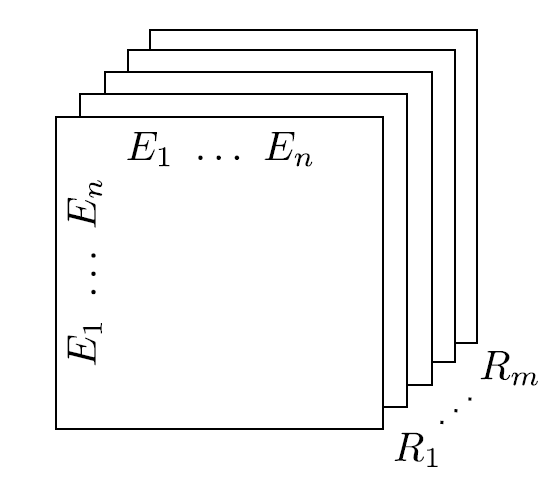
\includegraphics[width=.45\textwidth]{fig/embeddings/Rescal.png}
    \caption{Tensor representation of a Knowledge Graph with entities $E_1,...,E_n$ and relation $R_1,...,R_n$}
    \label{fig:emb-rescal}
\end{figure}

RESCAL applies a decomposition into directional components approach which is capable of detecting correlations between multiple interconnected nodes. It decomposes them into a 3-way tensor as shown in figure \ref{fig:emb-rescal}, two dimensions are generated by the concatenated entity vectors and the third represents the relations matrix.
In RESCAL, entities are expressed as vectors $v \in \mathbb{R}^d$ and relations are expressed as matrices $M \in \mathbb{R}^{d \times d}$  to calculate the score of a fact (h, r, t) a bilinear function is applied as defined by equation \ref{eq:rescal_scoring}.

\begin{equation}
    \label{eq:rescal_scoring}
    s(h, r, t) = v^T_h M_r v_t
\end{equation}

where $vh, vt \in \mathbb{R}^d$ are entity embeddings, and $M_r \in \mathbb{R}^{d\times d}$ is the matrix associated with the relations between them.

Continuing the work on tensor factorization we find DistMult \cite{}, an approach that tries to learn representations for entities and relations via a neural network in which the first layer projects a pair of input entities to low dimensional vectors, and the second layer combines them into a the input of the bilinear scoring function \ref{eq:distmult_scoring} which represents the relation between them looking to maximize this score.

\begin{equation}
    \label{eq:distmult_scoring}
    g^b_r (e1, e2) = e_1^T W_r e_2
\end{equation}

where $e_1$ and $e_2$ are the learned entity vectors and $W_r$ is the tensor operator. 

Furthering this line of work is complEx \cite{}, as suggested by the name instead of using embeddings containing real numbers it furthers the idea of complex embeddings, similarly to rotatE as seen previously. ComplEx argues that the standard dot product between embeddings can be a very effective composition function when using complex vectors.

This instance of the dot product involves the conjugate-transpose of one of the two vectors. As a consequence, the dot product is not symmetric any more, and facts about antisymmetric relations can receive different scores depending on the ordering of the entities involved.

Thus complex vectors can effectively capture antisymmetric relations while retaining the efficiency benefits of the dot product, that is linearity in both space and time complexity.

A key difference with the RotatE model which also focuses on these complex spaces is that ComplEx applies a tensor factorization approach in a bilinear way, this means that the same entity will have two different embedding vectors, depending on whether it appears as the subject or the object of a relation.

Finally the TuckER \cite{} model named after the author of Tucker decomposition \cite{} applies the principles of said technique to the tensor factorization model, by decomposing a tensor into a core tensor multiplied by a matrix along each mode as shown in figure \ref{fig:emb-tucker}, TuckER generalizes the problem presented in previous approaches.

\begin{figure}[!ht]
    \centering
    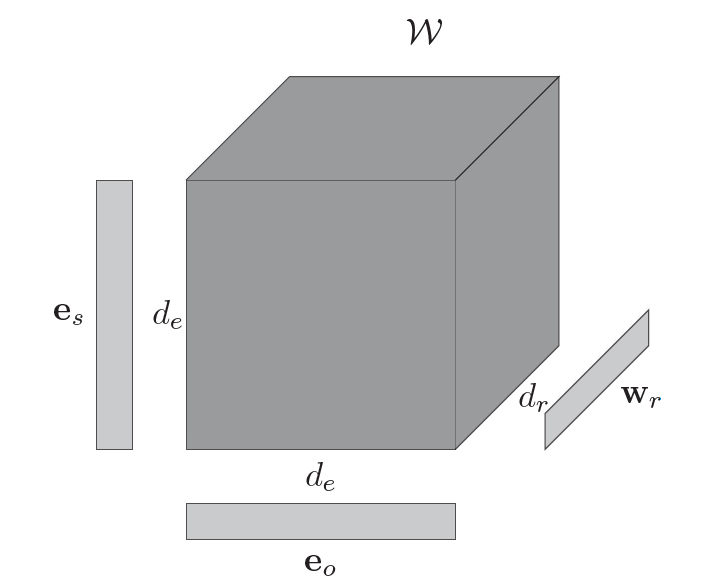
\includegraphics[width=.45\textwidth]{fig/embeddings/TuckER.png}
    \caption{TuckER architecture}
    \label{fig:emb-tucker}
\end{figure}

Using the Tucker decomposition for link prediction on the tensor representation of a knowledge graph, with entity embedding matrix $\mathcal{E}$ relation embedding matrix $\mathcal{R}$ the scoring function for this model is as shown in figure \ref{eq:tucker_scoring}

\begin{equation}
    \label{eq:tucker_scoring}
    \theta (h, r, t) = \mathbb{W} x_1 h x_2 w_r x_3 t
\end{equation}

where h, t are the rows of matrix $\mathcal{E}$ representing the subject and object entities vectors, $w_r$ the rows of the relation matrix and $\mathbb{W}$ is the core tensor to predict.

\section{Neural network-based models}\label{sec:emb-nn}

Neural networks can intelligently capture the semantic features of entities and relations and reasonably model the semantic relationships between discrete entities, which can help learn more accurate embeddings in the context of Knowledge Graphs problems. 

The improvement of Deep Neural Networks (DNNs), Recursive Neural Network (RNNs) or Graph Neural Networks(GNNs) along the previously discussed techniques made it an obvious path for research where NN models were tailored to generating this embedding representations of KG components. However NN models apply non-linear transformations to the data they are provided in which they lose explainability in the generative process.

One of the initial approaches for this method is Neural Tensor Networks (NTN) \cite{} it is a link prediction method which replaces a standard linear neural network layer with a bilinear tensor layer that directly relates two entity vectors across multiple dimensions making it so entities are represented as an average of their constituting word vectors. The model computes a score of how likely it is that two entities are in a certain relationship by the following NTN-based function shown in figure \ref{fig:emb-ntn}

\begin{figure}[!ht]
    \centering
    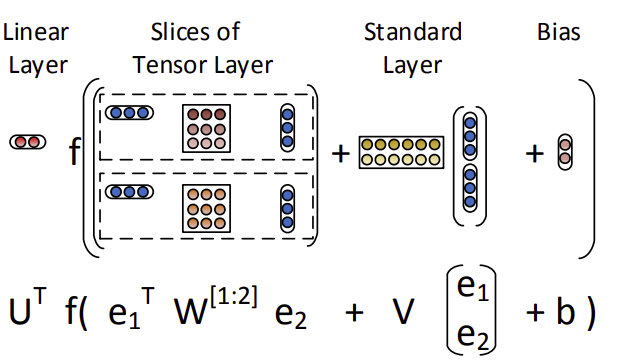
\includegraphics[width=.65\textwidth]{fig/embeddings/NTN.png}
    \caption{NTN layer}
    \label{fig:emb-ntn}
\end{figure}

ConvE \cite{} iterates upon the idea presented by NTN by using a multi-layer convolutional network model in order to be more parameter efficient than its predecessors and competitors such as DistMult. 

ConvE utilizes 2D convolutions over embeddings to predict missing links in knowledge graphs. It is the simplest multi-layer convolutional architecture for link  prediction. It is defined by a single convolution layer, a projection layer to the embedding dimension, and an inner product layer.

using a 2-dimensional convolution layer increases the expresiveness of the model as it increases the number of interaction points, thus being able to extract more feature interactions between two entity embeddings.

InteractE \cite{} improves upon ConvE by providing three key ideas feature permutation, a novel ``checkered'' feature reshaping, and circular convolution as the expressiveness of a model can be enhanced by increasing the possible interactions between embeddings.

\begin{figure}[!ht]
    \centering
    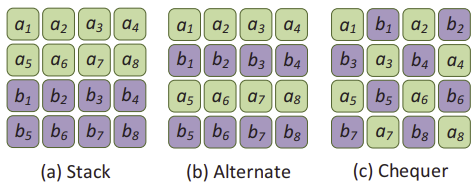
\includegraphics[width=.65\textwidth]{fig/embeddings/InteractE.png}
    \caption{InteractE checkered patter for tensor reshaping.}
    \label{fig:emb-interactE}
\end{figure}

\textit{Feature Permutation}: Instead of a fixed order for inputs InteractE allows for a mutable input order increasing the interaction between entity embeddings by allowing permutation between these inputs. However, the number of distinct interactions across all possible permutations is very large. So, for t different permutations, we can expect the total number of interactions to be approximately t times the number of interactions for one permutation.

\textit{Checkered Reshaping}: applies a reshape function for tensors that intertwines the features as seen in figure \ref{fig:emb-interactE}, which captures maximum heterogeneous interactions between entity and relation features.

\begin{figure}[!ht]
    \centering
    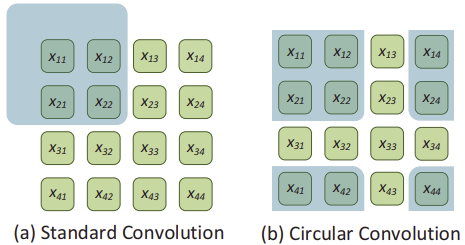
\includegraphics[width=.65\textwidth]{fig/embeddings/interactE_convolutions.png}
    \caption{InteractE circular convolution.}
    \label{fig:emb-interactE_conv}
\end{figure}

\textit{Circular Convolution}: Ciruclar convolution allows for a wraparound of the features selected for the convolution operation, as shown in figure \ref{fig:emb-interactE_conv}.

Also improving on ConvE we have ParamE, which makes use of translational properties such as the models in section \ref{sec:emb-translations} and neural networks non linear fitting skills such as previous models from this section.

\begin{figure}[!ht]
    \centering
    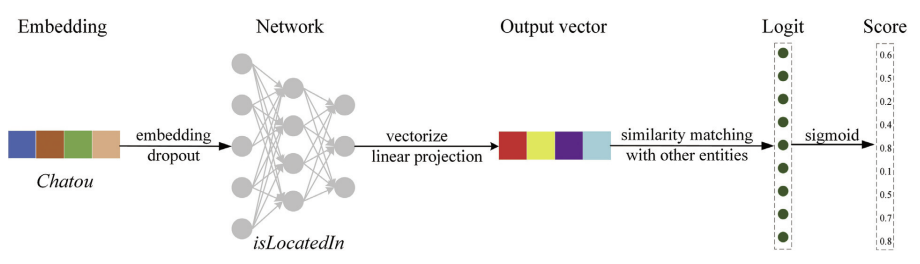
\includegraphics[width=\textwidth]{fig/embeddings/ParamE.png}
    \caption{ParamE model overview.}
    \label{fig:emb-paramE}
\end{figure}

In ParamE, head entity, relation, and tail entity embeddings are the input and output of a neural network respectively. taking neural network parameters as relation embeddings makes ParamE much more expressive and translational. entity and relation embeddings in ParamE belong to from feature space and parameter space respectively, which keeps them mapped into two different spaces. The main idea of ParamE is to regard NN parameters as relation embeddings, which makes it  expresive and translational.

ParamE is a general architecture for 3 separate NN models multilayer perceptrons,convolution layers, and gate structure layers, in which the latter is shown to outperform the other two measures.

Finally MEI \cite{} multi-partition embedding interaction model introduces the division of embeddings into multiple partitions, restricting the interactions in a triple to only entries in the corresponding embedding partitions of (h,r,t).

\begin{figure}[!ht]
    \centering
    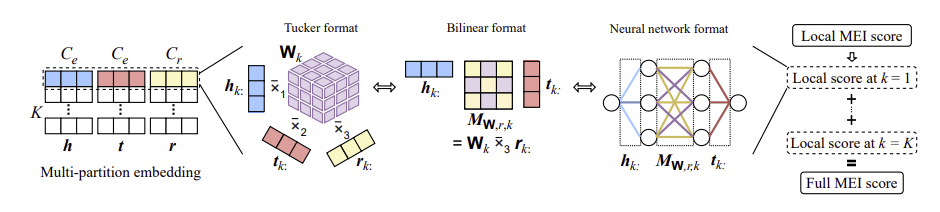
\includegraphics[width=\textwidth]{fig/embeddings/MEI.png}
    \caption{MEI model}
    \label{fig:emb-MEI}
\end{figure}

Interactions in each partition is done using the tucker format\cite{} to learn general linear interaction mechanisms figure \ref{fig:emb-MEI}. The total score for the model is the sum of all local interactions. 

In each triple (h, t, r), the entities and relations embedding vectors $h, t \in \mathbb{E}^{D_e}$ , and $r \in mathbb{R}^{D_r}$ are divided into multiple partitions, the score function of MEI \ref{eq:MEI_scoring} is defined as the sum score of $\mathcal{K}$ local interactions, with each local interaction being modeled by the Tucker format.

\begin{equation}
    \label{eq:MEI_scoring}
    \mathcal{S}(h, r, t; \theta) = \mathbb{W}_k x_1 h_k x_2 t_k x_3 r_k
\end{equation}

\section{Summary}\label{sec:emb-summary}
In this chapter, we have presented an overview of the existing methods that generate embedded representations of the information held in KGs. Particularly we have introduced and described the models that operate based on translation operations, to obtain numerical vectors that represent the information in KGs. We described several techniques based on the semantic information of each node within the graph. Also, we have overviewed the methods based on representing the KG as a third-order graph factorization model. Finally, we have enumerated the methods that use neural networks to generate these embeddings.